\documentclass[tikz,border=5pt]{standalone}
\usepackage[T1]{fontenc}
\usepackage[utf8]{inputenc}
\usepackage{lmodern}
\usepackage{amsmath,amssymb}
\usepackage{siunitx}
\usepackage{xcolor}
\usepackage{tikz}
\usetikzlibrary{
  arrows.meta,
  backgrounds,
  calc,
  decorations.pathreplacing,
  fit,
  matrix,
  positioning,
  shapes.geometric
}

\sisetup{
  detect-all = true,
  group-minimum-digits = 4,
}

\definecolor{TdcBlue}{HTML}{5B739F}
\definecolor{TdcRed}{HTML}{A35E66}
\definecolor{TdcLilac}{HTML}{8D83A7}
\definecolor{TdcCyan}{HTML}{82A9B8}
\definecolor{TdcGray}{HTML}{6D7175}
\definecolor{TdcBlack}{HTML}{202124}

\colorlet{TdcBlueFill}{TdcBlue!7}
\colorlet{TdcRedFill}{TdcRed!7}
\colorlet{TdcLilacFill}{TdcLilac!8}
\colorlet{TdcCyanFill}{TdcCyan!10}
\colorlet{TdcGrayFill}{black!3}
\colorlet{TdcGuide}{black!32}
\colorlet{TdcGuideLight}{black!18}

\tikzset{
  >=Latex,
  every picture/.style = {line join=round, line cap=round},
  every node/.style = {font=\small, text=TdcBlack},
  module/.style = {
    draw=black!72,
    fill=white,
    line width=0.50pt,
    rounded corners=0.8pt,
    minimum height=9mm,
    minimum width=22mm,
    align=center,
    inner sep=3pt
  },
  module gray/.style = {module, fill=TdcGrayFill},
  module slow/.style = {module, draw=TdcBlue, fill=TdcBlueFill},
  module fast/.style = {module, draw=TdcRed, fill=TdcRedFill},
  module ctrl/.style = {module, draw=TdcLilac, fill=TdcLilacFill},
  module io/.style = {module, draw=TdcCyan, fill=TdcCyanFill},
  domain box/.style = {
    draw=black!32,
    fill=black!1.5,
    line width=0.40pt,
    rounded corners=1.0pt,
    inner sep=4pt
  },
  domain label/.style = {
    font=\scriptsize\itshape,
    text=black!70
  },
  signal/.style = {-{Latex[length=2.2mm,width=1.5mm]}, draw=black!72, line width=0.60pt},
  signal slow/.style = {signal, draw=TdcBlue},
  signal fast/.style = {signal, draw=TdcRed},
  signal ctrl/.style = {signal, draw=TdcLilac},
  signal io/.style = {signal, draw=TdcCyan!80!black},
  signal dashed/.style = {signal, dashed},
  bidir/.style = {<->, draw=black!72, line width=0.55pt},
  guide/.style = {draw=TdcGuide, line width=0.35pt},
  guide dashed/.style = {guide, dashed},
  fine mark/.style = {draw=black!60, line width=0.40pt},
  brace note/.style = {
    decorate,
    decoration={brace, amplitude=3.0pt},
    draw=black!55,
    line width=0.40pt
  },
  note/.style = {
    font=\scriptsize,
    inner sep=1.5pt,
    fill=white,
    text=black!78
  },
  axis label/.style = {
    font=\scriptsize,
    text=black!72
  },
  lane label/.style = {
    font=\small,
    text=black!82
  },
  legend box/.style = {
    draw=black!60,
    line width=0.40pt,
    minimum width=4mm,
    minimum height=3mm
  },
  timeline block/.style = {
    draw=black!72,
    line width=0.45pt,
    minimum height=7.5mm,
    rounded corners=0.5pt,
    align=center,
    inner sep=2pt
  },
  timeline capture/.style = {timeline block, draw=TdcRed, fill=TdcRedFill},
  timeline snapshot/.style = {timeline block, draw=TdcLilac, fill=TdcLilacFill},
  timeline drain/.style = {timeline block, draw=TdcCyan!80!black, fill=TdcCyanFill},
  timeline free/.style = {timeline block, draw=black!60, fill=TdcGrayFill},
}

\newcommand{\DomainLabel}[2]{%
  \node[domain label, anchor=north west] at ($(#1.north west)+(0.10,-0.10)$) {#2};
}

\newcommand{\LegendItem}[4]{%
  \begin{scope}[shift={#1}]
    \node[legend box, fill=#2, anchor=west] at (0,0) {};
    \node[axis label, anchor=west] at (0.18,0) {#4};
  \end{scope}
}


\begin{document}
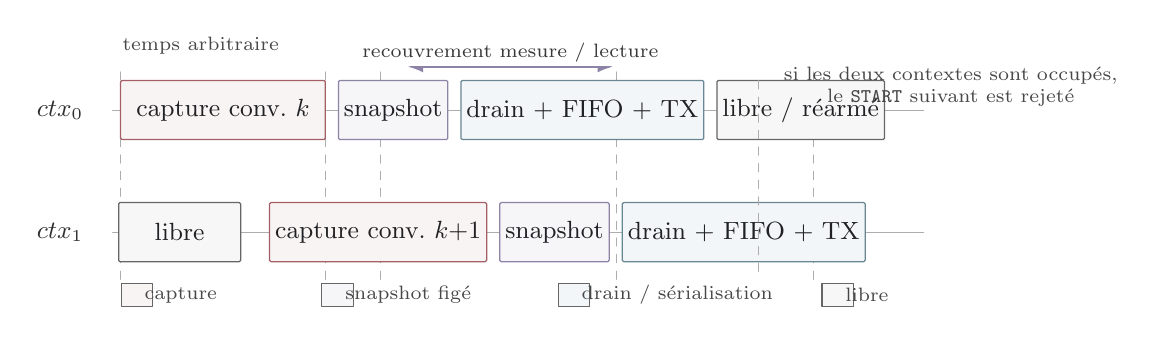
\begin{tikzpicture}[x=1cm,y=1cm]
  \draw[guide] (0.9,2.50) -- (11.2,2.50);
  \draw[guide] (0.9,0.95) -- (11.2,0.95);
  \node[lane label, anchor=east] at (0.65,2.50) {$ctx_0$};
  \node[lane label, anchor=east] at (0.65,0.95) {$ctx_1$};
  \node[axis label, anchor=west] at (0.90,3.32) {temps arbitraire};

  \foreach \x in {1.0,3.6,4.3,7.3,9.8} {
    \draw[guide dashed] (\x,0.35) -- (\x,3.05);
  }

  \node[timeline capture, minimum width=2.60cm] (c0cap) at (2.30,2.50) {capture conv.\ $k$};
  \node[timeline snapshot, minimum width=0.95cm, right=0.15cm of c0cap] (c0snap) {snapshot};
  \node[timeline drain, minimum width=2.85cm, right=0.15cm of c0snap] (c0drain) {drain + FIFO + TX};
  \node[timeline free, minimum width=2.00cm, right=0.15cm of c0drain] (c0free) {libre / réarmé};

  \node[timeline free, minimum width=1.55cm] (c1free0) at (1.75,0.95) {libre};
  \node[timeline capture, minimum width=2.45cm, right=0.35cm of c1free0] (c1cap) {capture conv.\ $k{+}1$};
  \node[timeline snapshot, minimum width=0.95cm, right=0.15cm of c1cap] (c1snap) {snapshot};
  \node[timeline drain, minimum width=2.75cm, right=0.15cm of c1snap] (c1drain) {drain + FIFO + TX};

  \draw[bidir, draw=TdcLilac] (4.65,3.05) -- node[note, above] {recouvrement mesure / lecture} (7.25,3.05);
  \draw[guide dashed] (9.1,0.45) -- (9.1,2.95);
  \node[axis label, align=center, anchor=west] at (9.30,2.80)
    {si les deux contextes sont occupés,\\le \texttt{START} suivant est rejeté};

  \LegendItem{(1.00,0.15)}{TdcRedFill}{TdcRed}{capture}
  \LegendItem{(3.55,0.15)}{TdcLilacFill}{TdcLilac}{snapshot figé}
  \LegendItem{(6.55,0.15)}{TdcCyanFill}{TdcCyan}{drain / sérialisation}
  \LegendItem{(9.90,0.15)}{TdcGrayFill}{black!60}{libre}
\end{tikzpicture}
\end{document}
